\newpage
\section{De Morgan dependencies for brushing and linking}
\label{sec:de-morgan}

\secref{data-dependencies} addresses the first kind of question we motivated in the introduction (\secref{introduction:data-linking}). In particular $\evalBwdF{T}$ can answer questions like: ``what data is needed to compute this bar in a bar chart?'', and indeed we were able to use our implementation to generate \figref{introduction:data-linking}. The second problem we set ourselves was how to link selections between \emph{cognate} outputs, i.e.~outputs computed from the same data~(\secref{introduction:vis-linking}). This is called ``brushing and linking'' \cite{becker87} in data visualisation, and has been extensive studied as an interaction paradigm, but with little emphasis of techniques for automation. Intuitively, the problem has a bidirectional flavour: one must consider how dependencies flow backward from a selection in one output to a selection $v$ in the common data, and then forward from the selected data $v$ to a corresponding selection in the other output. A natural question then is whether the analysis established in \secref{data-dependencies} can supply the information required to support an automated solution.

An immediate problem is that the flavour of the forward dependency required here differs from that provided by the forward analysis $\evalFwdF{T}$ defined in \secref{data-dependencies:analyses:fwd}. That was able to answer the question: what can we compute given only the data selected in $v$? But to identify the related data in another output, we must determine not what the input selection $v$ is sufficient for, but what it is necessary for: those parts of the other output that depend on $v$. In fact the question can be formulated as a kind of dual: what would we \emph{not} be able to compute if the data selected in $v$ were \emph{unavailable}?

\subsection{De Morgan duality}
\label{sec:de-morgan:de-morgan-duality}

Why $\evalFwdF{T}$ is unsuitable as a forward dependency relation for linking cognate outputs can also be understood in terms of compositionality. Suppose $\Ann{V}_1$ and $\Ann{V}_2$ are the lattices of selections for two views computed from a shared input source, and $\Ann{D}$ is the lattice of selections for the shared input. Using the procedure given in \secref{data-dependencies}, we can obtain two Galois connections $f: \Ann{V}_1 \to \Ann{D}$ and $g: \Ann{V}_2 \to \Ann{D}$ as shown in \figref{example:de-morgan:non-composable} below; we ask the reader to ignore \figref{example:de-morgan:composable} for the moment.

\begin{figure}[H]
   \begin{subfigure}[t]{0.43\textwidth}
      \begin{nscenter}
         \begin{tikzpicture}[node distance=1.5cm, auto]
            \node (AA) [node distance=2cm] {
               $\Ann{V}_1$
            };
            \node (BB) [right of=AA] {
               $\Ann{D}$
            };
            \node (CC) [right of=BB] {
               $\Ann{V}_2$
            };
            \node (A) [below of=AA] {
               $\Ann{V}_1$
            };
            \node (B) [right of=A] {
               $\Ann{D}$
            };
            \node (C) [right of=B] {
               $\Ann{V}_2$
            };
            \draw[->] (AA) to node {$f$} (BB);
            \draw[->] (CC) to node [swap] {$g$} (BB);

            \draw[->, bend right] (A) to node [swap] {$\lowerAdj{f}$} (B);
            \draw[->, bend left] (B) to node {$\upperAdj{g}$} (C);
            \draw[->, bend left] (C) to node {$\lowerAdj{g}$} (B);
            \draw[->, bend right] (B) to node [swap] {$\upperAdj{f}$} (A);

            \draw[red,thick,dotted,line cap=round,dash pattern=on 0pt off 0.2em] ($(BB.north west)+(0.1,0.3)$)  rectangle ($(C.south east)+(-0.1,-0.5)$);
         \end{tikzpicture}
      \end{nscenter}
      \caption{Non-composable Galois connections}
      \label{fig:example:de-morgan:non-composable}
   \end{subfigure}
   \begin{subfigure}[t]{0.55\textwidth}
      \begin{nscenter}
         \begin{tikzpicture}[node distance=1.5cm, auto]
            \node (AA) [node distance=2cm] {
               $\Ann{V}_1$
            };
            \node (BB) [right of=AA] {
               $\Ann{D}$
            };
            \node (CC) [right of=BB] {
               $\Ann{V}_2$
            };
            \node (A) [below of=AA] {
               $\Ann{V}_1$
            };
            \node (A1) [right of=A] {
               $\Ann{D}$
            };
            \node (B) [right of=A1] {
               $\Ann{D}$
            };
            \node (C) [right of=B] {
               $\Ann{V}_2$
            };
            \node (C1) [right of=C] {
               $\Ann{V}_2$
            };
            \draw[->] (AA) to node {$f$} (BB);
            \draw[->] (BB) to node {$\dual{g}$} (CC);

            \draw[->, bend right] (A) to node [swap] {$\lowerAdj{f}$} (A1);
            \draw[->, bend right] (A1) to node [swap] {$\neg_{\Ann{D}}$} (B);
            \draw[->, bend right] (B) to node [swap] {$\upperAdj{g}$} (C);
            \draw[->, bend right] (C) to node [swap] {$\neg_{\Ann{V}_2}$} (C1);
            \draw[->, bend right] (C1) to node [swap] {$\neg_{\Ann{V}_2}$} (C);
            \draw[->, bend right] (C) to node [swap] {$\lowerAdj{g}$} (B);
            \draw[->, bend right] (B) to node [swap] {$\neg_{\Ann{D}}$} (A1);
            \draw[->, bend right] (A1) to node [swap] {$\upperAdj{f}$} (A);

            \draw[red,thick,dotted,line cap=round,dash pattern=on 0pt off 0.2em] ($(BB.north west)+(0.1,0.3)$)  rectangle ($(C1.south east)+(-0.1,-0.5)$);
         \end{tikzpicture}
   \end{nscenter}
   \caption{Composing via De Morgan duality}
   \label{fig:example:de-morgan:composable}
\end{subfigure}
\caption{Dualising $g: \Ann{V}_2 \to \Ann{D}$ for composition with $f: \Ann{V}_1 \to \Ann{D}$}
\end{figure}

\vspace{-1mm}

\noindent Unfortunately, $f$ and $g$ are not composable, as their types makes clear. While the upper adjoint $\upperAdj{g}: \Ann{D} \to \Ann{V}_2$ has the correct type to compose with the lower adjoint $\lowerAdj{f}: \Ann{V}_1 \to \Ann{D}$, the result is not a Galois connection: $\upperAdj{g}$ preserves meets, whereas $\lowerAdj{f}$ preserves joins. However, it turns out that if selections are closed under complement, we can derive an analysis of what is \emph{necessary} for a given input selection from an analysis of what it is \emph{sufficient} for. The effect is to invert $g$, yielding a Galois connection $\dual{g}$ with a type that allows it to compose with $f$. Then the composite $\dual{g} \after f$ is a Galois connection linking $\Ann{V}_1$ to $\Ann{V}_2$ via $\Ann{D}$, as shown in \figref{example:de-morgan:composable}, providing a general mechanism for brushing and linking, with nice round-tripping properties. We now unpack this in more detail.

First we shift settings from the lattices used in \secref{data-dependencies} to Boolean lattices (or Boolean algebras) $\Ann{A}= \BoolLattice{\Ann{A}}{\top}{\bot}{\meet}{\join}{\neg}$, which are lattices equipped with an involution $\neg: \Ann{A} \to \Ann{A}$ called \emph{complement}. Boolean algebras satisfy complementation laws $x \meet \neg x = \bot$ and $x \join \neg x = \top$ and De Morgan laws $\neg x \meet \neg y = \neg(x \join y)$ and $\neg x \join \neg y = \neg(x \meet y)$. If $\Ann{A}$ is a Boolean algebra, then $\Sel{\raw{v}}{A}$ is also a Boolean algebra, with the Boolean operations, and in particular $\neg_{\raw{v}}: \Sel{\raw{v}}{A} \to \Sel{\raw{v}}{A}$, defined pointwise. An additional distinguished selectable value $\blackhole$ serves as the negation of $\hole$. The two-point lattice $\Bool$ we used to illustrate \secref{data-dependencies} is also a Boolean algebra $\BoolLattice{\Bool}{\TT}{\FF}{\wedge}{\vee}{\neg}$ with $\neg$ corresponding to logical negation.

\begin{figure}[b]
   \hspace{0.11in}
   \begin{subfigure}[t]{2.9in}
      \small
      \lstinputlisting[language=Fluid]{fluid/convolution.fld.mod}
   \end{subfigure}
   \hspace{0.3in}
   \begin{subfigure}[t]{2.05in}
      \small
      \lstinputlisting[language=Fluid]{fluid/conv-emboss.fld.mod}
   \end{subfigure}
   \caption{Matrix convolution example, with methods \kw{zero}, \kw{wrap} and \kw{extend} for dealing with boundaries}
   \label{fig:example:convolve}
\end{figure}


It is an easy consequence of the complementation and De Morgan laws that any meet-preserving operation $g: \Ann{A} \to \Ann{B}$ on Boolean algebras has a join-preserving De Morgan dual $\dual{g}: \Ann{A} \to \Ann{B}$ given by $\neg_{\Ann{B}} \after g\after \neg_{\Ann{A}}$, and any join-preserving operation $h$ has a meet-preserving De Morgan dual $\dual{h}$ defined similarly. Moreover if $h$ is the lower adjoint of $g$, then $\dual{g}$ is the lower adjoint of $\dual{h}$. Thus Galois connections on Boolean algebras also admit a (contravariant) notion of De Morgan duality, defined component-wise.

\begin{definition}[De Morgan dual of a Galois connection]
   Suppose $\Ann{A}$ and $\Ann{B}$ are Boolean algebras and $f: \Ann{A} \to \Ann{B}$ is a Galois connection $(\lowerAdj{f},\upperAdj{f})$. Define the \emph{De Morgan dual} $\dual{f}$ of $f$ to be the Galois connection $(\dual{\upperAdj{f}}, \dual{\lowerAdj{f}}): \Ann{B} \to \Ann{A}$.
\end{definition}

\noindent Dualising a Galois connection flips the direction of the arrow by swapping the roles of the upper and lower adjoints. So while $f: \Ann{A} \to \Ann{B}$ and $g: \Ann{C} \to \Ann{B}$ are not composable, $f$ and $\dual{g}: \Ann{B} \to \Ann{C}$ are, and the composition is achieved by transforming $\upperAdj{g}$ from something which determines what we can compute with $v$ into something which determines what we cannot compute without $v$. This offers a principled basis for an automated brushing and linking feature between cognate computations $T$ and $U$. When the user selects part of the output of $T$, we can use $\evalBwdF{T}$ to compute the needed data $v$, and then use $\dual{\evalFwdF{U}}$ to compute the parts of the output of $U$ that depend on $v$. This is the approach implemented in \OurLanguage, which we used to generate \figref{introduction:vis-linking} in \secref{introduction:vis-linking}.

\subsection{Example: matrix convolution}
\label{sec:de-morgan:example}

We now illustrate the $\dual{\evalGC{T}}$ Galois connection, contrasting it with $\evalGC{T}$, using an example which computes the convolution of a $5 \times 5$ matrix with a $3 \times 3$ kernel. Convolution has an intuitive dependency structure and the values involved have an easy visual presentation, making it useful for conveying the flavour of the four distinct (but connected) dependency relations that arise in the framework. The source code for the example is given in \figref{example:convolve}, and shows the \kw{convolve} function, plus \kw{zero}, \kw{wrap} and \kw{extend} which provide different methods for handling the boundaries of the input matrix. The angle-bracket notation is used to construct matrices, which were omitted from \secref{core-language}. (The formal treatment is similar to records.)

\begin{figure}
   \begin{subfigure}{0.53\textwidth}
      {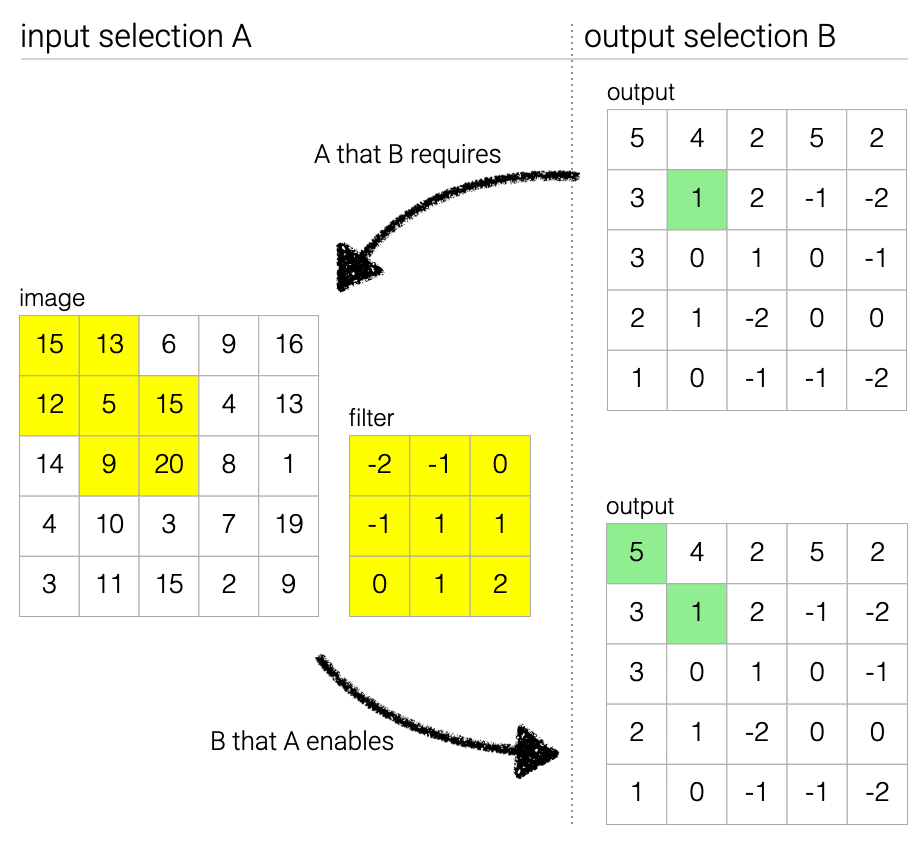
\includegraphics[scale=0.4]{fig/example/4-relations-1.png}}
      \vspace{2mm}
      \caption{Galois dependency $(\evalBwdF{T}, \evalFwdF{T})$}
      \label{fig:example:convolve-viz:galois-dependency}
   \end{subfigure}
   \begin{subfigure}{0.46\textwidth}
      {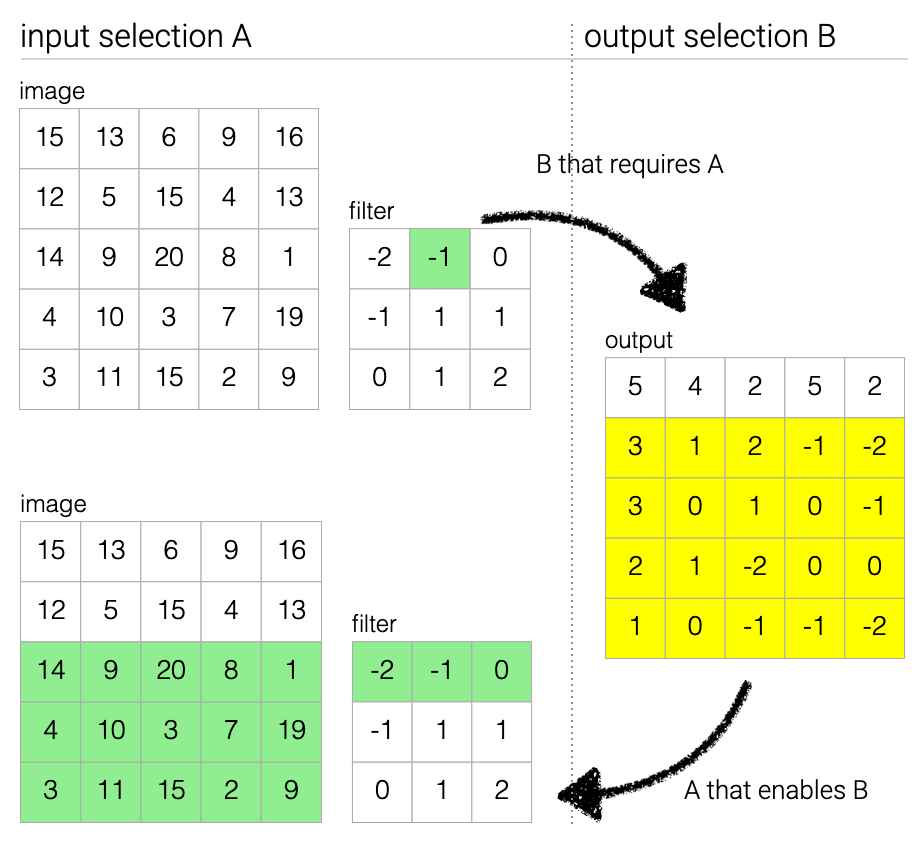
\includegraphics[scale=0.4]{fig/example/4-relations-2.png}}
      \vspace{2mm}
      \caption{De Morgan dual $(\dual{\evalFwdF{T}}, \dual{\evalBwdF{T}})$}
      \label{fig:example:convolve-viz:de-morgan-dual}
   \end{subfigure}
   \caption{Upper and lower pairs are dual; left and right pairs are adjoint}
   \label{fig:example:convolve-viz}
\end{figure}


\OurLanguage{} was used to generate the diagrams in \figref{example:convolve-viz}, which show the four dependency relations and two of their four possible round-trips. \figref{example:convolve-viz:galois-dependency} shows the $\evalGC{T}$ Galois connection defined in \secref{data-dependencies:galois-connections}. In the upper figure, the user selects (in green) the output cell at position $(2,2)$ (counting rows downwards from $1$). This induces a demand (via the lower adjoint $\evalBwdF{T}$) on the input matrix \kw{image} and the kernel \kw{filter}, revealing (in yellow) that the entire kernel was needed to compute the value $1$, but only some of the input matrix. In particular the elements at $(1,3)$ and $(3,1)$ in \kw{image} were not needed, because of zeros present in \kw{filter}. If we then ``round-trip'' that input selection, computing the corresponding availability on the output using the upper adjoint $\evalFwdF{T}$, the green selection grows: it turns out that the data needed to make $(2,2)$ available are sufficient to make $(1,1)$ available as well.

\figref{example:convolve-viz:de-morgan-dual} shows the De Morgan dual $\dual{\evalGC{T}}$. In the upper part of the figure, the user selects (green) kernel cell $(1, 2)$ to see the output cells that depend on it. This is computed using the De Morgan dual of $\evalFwdF{T}$. First we negate the input selection, marking $(1, 2)$ as unavailable, and all other inputs as available. Then we forward-analyse with $\evalFwdF{T}$ to determine that with this data selection, we can only compute the top row of the output. (If it seems odd that we can compute even the top row, notice that the example uses the method \kw{zero} for dealing with boundaries; \kw{wrap} or \kw{extend} would give a different behaviour.) Then we negate that top row selection to produce the (yellow) output selection shown in the figure. These are exactly the output cells which depend on kernel cell ($1, 2)$ in the sense that they cannot be computed if that input is unavailable.

We can then round-trip this output selection using the De Morgan dual of $\evalBwdF{T}$. We first negate the yellow output selection (selecting the top row of the output again), and then use $\evalBwdF{T}$ to determine the needed inputs, which turn out to be the top two rows of \kw{image}, and the top row of \kw{filter}. Negating again produces the green output selection shown in the lower figure. Thus the backwards De Morgan dual computes the inputs that would \emph{not} be needed if the selected outputs were not needed: more economically, the inputs that are \emph{only} needed for the selected output. Here the round-trip reveals that if kernel cell $(1, 2)$ is unavailable, then the entire top row of the kernel might as well have been unavailable too, and similarly for the bottom 3 rows of the input.

\subsection{Relationship to Galois slicing}
\label{sec:de-morgan:galois-slicing}

\begin{figure}
   \small
   \begin{centering}
      \begin{subfigure}{0.45\textwidth}
         {\lstinputlisting[language=Fluid,escapeinside={(*@}{@*)}]{other-src/diff-slicing-0.example}}
      \caption{Original program}
      \label{fig:example:diff-slicing:original}
      \end{subfigure}
      \begin{subfigure}{0.45\textwidth}
         {\lstinputlisting[language=Fluid,escapeinside={(*@}{@*)}]{other-src/diff-slicing-2.example}}
      \caption{Backward slice for \kw{(0.4, $\hole$)}}
      \label{fig:example:diff-slicing:subtree}
      \end{subfigure}
      \\
      \begin{subfigure}{0.45\textwidth}
         {\lstinputlisting[language=Fluid,escapeinside={(*@}{@*)}]{other-src/diff-slicing-1.example}}
      \caption{Backward slice for spine \kw{($\hole$, $\hole$)}}
      \label{fig:example:diff-slicing:spine}
      \end{subfigure}
      \begin{subfigure}{0.45\textwidth}
         {\lstinputlisting[language=Fluid,escapeinside={(*@}{@*)}]{other-src/diff-slicing-3.example}}
      \caption{Differential backward slice for \kw{(\codeSelTwo{0.4}, $\hole$)}}
      \label{fig:example:diff-slicing:differential}
      \end{subfigure}
   \end{centering}
   \vspace{-2mm}
   \caption{Differential Galois slicing selects input (blue) needed \emph{only} for selected output (green)}
   \label{fig:example:diff-slicing}
\end{figure}


The De Morgan dual puts us in a better position to consider the relationship between the present system and earlier work on \emph{Galois slicing}, a program slicing technique that has been explored for pure functional programs~\cite{perera12a}, functional programs with effects~\cite{ricciotti17}, and \piCalculus~\cite{perera16d}. We consider other related work in \secref{conclusion}.

Galois slicing operates on lattices of \emph{slices}, which are programs (or values) where parts deemed irrelevant are replaced by a hole $\hole$. (If we think of the notion of selection defined in \secref{data-dependencies:selections} as picking out a subset of the paths in a term, then slices resembles selections which are prefix-closed, meaning that if a given path in a term is selected, then so are all of its prefixes.) For a fixed computation, a meet-preserving \emph{forward-slicing} function is defined which takes input slices to output slices, discarding parts which cannot be computed because the needed input is not present, plus a join-preserving \emph{backward-slicing} function taking output slices to input slices, retaining the parts needed for the output slice. For example \figref{example:diff-slicing:original} shows a computation with output \lstinline{(0.4, 0.6)}, and \figref{example:diff-slicing:subtree} gives the backward slice for output slice \kw{(0.4, $\hole$)}. Forward and backward slicing, for a given computation, form a Galois connection, giving the analyses the nice round-tripping properties we motivated in \secref{data-dependencies:galois-connections}.

Unfortunately, the notion of slice does not lend itself to computing dependencies where the needed input or output is a proper part of a value, such as a component of a tuple. \emph{Differential} slicing \cite{perera12a} improves on this by using Galois slicing to compute a pair of input slices $(e,e'$) for a pair of output slices $(v,v')$ where $v \leq v'$. By monotonicity, $e \leq e'$. This can be used to compute a (differential) slice for an arbitrary subtree, by setting $v$ to be the ``spine'' of the original output up to the location of the subtree, and $v'$ to be $v$ with the subtree of interest plugged back in. Here we could focus on the value \kw{0.4} in the output by computing the backward slice for $\kw{($\hole$, $\hole$)}$ (\figref{example:diff-slicing:spine}) and then comparing it with the backward slice for \kw{(0.4, $\hole$)}, generating a differential slice where the parts that are different are highlighted (\figref{example:diff-slicing:differential}). But although it supports a notion of selection which is closer to what we need, the differential slice highlights only the program parts that are needed \emph{exclusively} by the selected output. Here, \lstinline{2} and \lstinline{3} are needed to compute the spine as well (in order to decide which conditional branch to execute), so they are excluded from the differential slice. In fact differential slicing is similar to the dual of $\evalBwdF{T}$, and as such underapproximates the dependency information needed for data linking.
